\documentclass{article}
\usepackage[a4paper, landscape, top = 2cm, bottom = 2cm, left = 2cm, right = 2cm]{geometry}
\usepackage{multicol}
\usepackage{bm}
\usepackage{xcolor}

\usepackage{graphicx}\usepackage{lmodern}

\usepackage[sc]{mathpazo} % Use the Palatino font
\usepackage[utf8]{inputenc}
\usepackage[T1]{fontenc}
\linespread{1.05} % Line spacing - Palatino needs more space between lines
\usepackage{microtype} % Slightly tweak font spacing for aesthetics
\setlength\parindent{0pt}
%\usepackage{textgreek}

\usepackage{fancyhdr} % Headers and footers
\pagestyle{fancy} % All pages have headers and footers
\fancyhead{} % Blank out the default header
\fancyfoot{} % Blank out the default footer
\fancyhead[C]{Róbert Jurčo \hfill Classical and theoretical mechanics cheatsheet} % Custom header text
\fancyfoot[C]{\thepage} % Custom footer text

\usepackage{amsmath, amssymb, amsfonts, amsthm, wasysym}
\newcommand{\N}{\mathbb{N}}
\newcommand{\Z}{\mathbb{Z}}
\newcommand{\Q}{\mathbb{Q}}
\newcommand{\R}{\mathbb{R}}
\newcommand{\C}{\mathbb{C}}

\renewcommand\d{\mathrm d}

\DeclareMathOperator{\arccot}{arccot}
\DeclareMathOperator{\arcsinh}{arcsinh}
\DeclareMathOperator{\arccosh}{arccosh}
\DeclareMathOperator{\arctanh}{arctanh}
\DeclareMathOperator{\arccoth}{arccoth}


\begin{document}
\begin{multicols}{3}
    \textbf{{\color{red} DO: Vector identities cheatsheet}}

    \textbf{{\color{red} DECIDE: Use bold or vector ntation?}}

    \textbf{{\color{red} REDO: }General concepts and skills}

    \begin{enumerate}

        \item numerical methods: Euler $y_{i+1}=y_i+f(t_i,y_i)\Delta t$

    \end{enumerate}

    \textbf{{\color{red} REDO: }Data analysis}

    \textbf{{\color{red} REDO: }Mathematicasa}

    \begin{enumerate}
        \item $\frac{d}{dt}\int_0^tf(x)dx=f(t)+\int_0^t\frac{t}{dt}f(x)dx$
        \item Derivations: \\
            $\frac{\d}{\d x}\arcsin(x)=\frac{1}{\sqrt{1-x^2}}$,
            $\frac{\d}{\d x}\arccos(x)=\frac{-1}{\sqrt{1-x^2}}$\\
            $\frac{\d}{\d x}\arctan(x)=\frac{1}{1+x^2}$,
            $\frac{\d}{\d x}\arccot(x)=\frac{-1}{1+x^2}$\\
            $\frac{\d}{\d x}\arcsinh(x)=\frac{1}{\sqrt{x^2+1}}$,
            $\frac{\d}{\d x}\arccosh(x)=\frac{1}{\sqrt{x^2-1}}$\\
            $\frac{\d}{\d x}\arctanh(x)=\frac{1}{1-x^2}$ and $1>x^2$\\
            $\frac{\d}{\d x}\arccoth(x)=\frac{1}{1-x^2}$ and $1<x^2$
        \item Fourier: \\
            $f(x)=\sum c_ne^{inx}$ where $c_n=\frac{1}{2\pi}\int_0^{2\pi}f(x)e^{-inx}dx$
        \item Dot and Cross products are distributive.
        \item $\nabla\cdot(\nabla\times\vec{A})=0$ and
            $\nabla\times(\nabla f)=0$
        \item Triple product $\vec{A}\cdot(\vec{B}\times\vec{C}) =\vec{B}\cdot(\vec{C}\times\vec{A})
         =\vec{C}\cdot(\vec{A}\times\vec{B})$
         $=\begin{vmatrix}
             A_x & A_y & A_z \\
             B_x & B_y & B_z \\
             C_x & C_y & C_z
         \end{vmatrix}$
        \item BAC-CAB rule: $\vec{A}\times(\vec{B}\times\vec{C})
         =\vec{B}(\vec{A}\cdot\vec{C})-\vec{C}(\vec{A}\cdot\vec{B})$
    \end{enumerate}

    \centering{\large\textbf{I. KINEMATICS}}

    \begin{enumerate}
        \item $\vec v=\d\vec x/\d t$, $\vec a=\d\vec v/\d t$, $t=\int v_x^{-1}\d x=\int a_x^{-1}\d v_x$, $x=\int v_x/a_x\d v_x$, where integrals could be found from plot as an area under graph.
        \item If $a=Const.$, then: $x=(v^2-v_0^2)/2a$.
        \item {\color{red} Do we want here eqs. for movement in g field?}
        \item Rotational motion: $\omega=d\phi/dt\text,\quad\epsilon=d\omega/dt$\\$\vec a=\d v/\d t\hat{e}_\tau+v^2/R\hat{e}_n$
        \item Motion of a rigid body. \textbf{a)} $v_a\cos\alpha=v_b\cos\beta$; $\vec{v_a}\text{, }\vec{v_b}$ --- velocities of points A and B;
            \textbf{b)} The instanteous center of rotation can be found as the intersection pt. of perpediculars to $\vec{v_a}$ and $\vec{v_b}$ from the points A and B, or(if $\vec{v_a}, \vec{v_b}\bot AB$) as the ntersection pt. of AB whith the line connecting endpoints of $v_a$ and $v_b$
        \item Centrifugal force $\vec F=m\omega^2\vec r$, Coriolis force $\vec{F} = m\vec{v}\times\vec{\omega}$
        \item Ballistic problem reachable region \par
            $y\leq v_0^2/(2g)-gx^2/(2v_0^2)$\par
            For and optimal balistic trajectory, initial and final velocities are perpendiculars.
        \item Parabola is equidistant from focus and directrix (or use line parallel to direcrtix passing throught focus). Rays parallel to y-axis are reflected to focal point.
        \item Elastic bounce of ball from moving wall:\\
            $\vec v_n\:'=-\vec v_n+2\vec u$
        \item For findings fastest paths, Snell's, Fermat's and Huygen's principles can be used.
        \item To find a vector (velocity, acceleration) its enought to find its direction and projection to single axes.
        \item Methods of solving prob.: Vector and Geometry, Differentiat. approach (calc. infinitezimal change of system), Equations of motion, Investigation in specific frame.
    \end{enumerate}
    ~\\~\\~\\
    \centering{\large\textbf{II. STATICS}}

    \begin{enumerate}
        \item For a 2D equilibrium of a rigid body: 2 eqns. for Forces, 1 eq. for torque. 1(2) eq. for force can be substituted whith 1(2) for torque. Torque is often better then boring forces.
        \item Normal and frictional force can be combined into a sngle force, applied under $arctan\,\mu$ with respect to the normal.
        \item $F_t\leq\mu mg$, there are several types: static, kinetic (sliding, dynamic).
        \item Pulleys: a) Force in pulley axis = $\Sigma$ forces from rope.\\
            b) $\Sigma$ of center shifts of all the rope parts = 0\\
            c) If you draw a line through system of pulleys, then $\Sigma$ of forces "acting" on the line is in the equilirium zero.
            d) Virtual work ~~~e) Noether theorem
        \item Virtual work: in equilibrium\\ $\delta W=\Delta \Pi-\Sigma F\Delta x =0$
        \item For studying stability (instability) use principle of minimum (maximum/saddle point) of potential energy or principle of virtual work (small displacement).
    \end{enumerate}

    \centering{\large\textbf{III. LAWS OF CONSERVATION}}

    \begin{enumerate}
            \item Momentum: no net external forces or conseved along axis $\perp$ to the net external force.
            \item Energy: elastic bodies, no friction, conservative fields $\nabla\times\vec F=0$
            \item Angular momentum: no net external torque (arm = 0), can be written rel. to 2(3) pts. then substitutes conservation of lin. mom.
            \item Number of nucleons and total charge.
    \end{enumerate}

    \centering{\large\textbf{IV. DYNAMICS}}
    \begin{enumerate}

        \item Newton's 1 law: There exists a frame of reference (called inertial), in which each isolated point mass moves uniformly in a straight line.
        \item Newton's 2 law: For each point mass there exists a constant $m$ and a vector function $\vec F$ such that its motion with respect to the inertial system is given by $m\ddot{\vec{x}} =\vec F$, $\left(\vec F_\Sigma=\d\vec p/\d t\right)$.
        \item Mass accretion ($\d m>0$) / ejection: ($\d m<0$) $m\vec a=\vec F_{ext}+\vec v_{rel}\frac{dm}{dt}$.
        \item Index C denotes quantities rel. to the centre of mass:
            $\vec P_C=\sum m_i\vec v_i$, $K=\sum m_iv_i^2/2$\\ $\vec P_i=\vec P_{Ci}-M_\Sigma\vec v_C$, $K_i=K_{Ci}+M_\Sigma v_C^2/2$
        \item If forces are applied only to 2 points, the net force application lines coincide; for 3 points, the lines meet at a single point.
        \item Tilted coordinates (motion on an inclined plane).
        \item Generalized coordinate $q$:\\ $\mathcal M\ddot q =-\d\Pi(q)/\d q$ and $T =\mathcal M\dot{q}^2/2$
        \item Non-inertial frames of ref.: inertial force $-m\vec a$, centrifugal force $m\omega^2\vec r$, Coriolis force $2m\vec v\times\vec \Omega$ (better to avoid it, it does not create any work)
        \item Stoke's drag: force of viscosity on a small sphere moving through a viscous fluid $F=6\pi\eta Rv$
        \item Drag equation: $F=\rho CSv^2/2$, where $\rho$ - density of the fluid, $S$ - reference area, $C$ - drag coeficient.
        \item Collision of 2 bodies: conserved are\\
            a) net momentum b) net angular mom.\\
            c) total enery (for elastic collisions)\\
            d) if sliding stops during the impact, final velocities of the contact points will have equal projections to the contact plane;\\
            e) if sliding doesn't stop, the momentum delivered during the impact froms angle $arctan\,\mu$ with the normal.
        \item Tension $T$ in a string: horizontal component is conctant, vertical $\propto$ mass underneath. On pulley with friction tension change $e^{\mu\phi}$ times. Presure force $N$ per unit lenght (resting on a smooth surface) is $\propto$ its radius R: $N=T/R$
        \item Adiabatic invariant: if a relative change of an oscillating system is small during one period, the area I of the loop drawn in p-x coordinates is conversed with a very high accuracy.
        \item Continuity condition: $\d m/\d t=\rho Sv$

    \end{enumerate}

    \centering{\large\textbf{V. ROTATIONAL MOTION}}

    \begin{enumerate}
        \item $\vec\tau =I\vec\epsilon=\d\vec L/\d t$, where $\vec L=\sum\vec r_i\times\vec P_i$
        \item $\vec L=I\vec\omega$, $\vec L=\sum m_i\vec r_i\times\vec v_i$, $\vec L_i=\vec L_{Ci}+M_\Sigma\vec R_C\times\vec v_C$
        \item Point masses \& fixed origin: $\vec\tau=\vec r\times\vec F^{ext}$
        \item System of point masses \& fixed origin:\\ $\vec\tau=\sum\vec r_i \times\vec F_i^{ext}$
        \item System of point masses \& non-fixed origin:\\$\vec\tau=\sum(\vec r_i-\vec r_0)\times\vec F_i^{ext}-(\vec r_C-\vec r_0)\times (M_C \ddot r_0)\hat r_0$\\There are 3 cases when the second term is zero.
        \item Rotation of body can be discribed by ortogonal ($A^T=A^{-1}$) matrix $A_{ij}(t)$ such, that $\hat e'_i=A_{ij}\hat e_j$, where $\hat e'_i$ is co-rotating and $\hat e_j$ inertial basis.
        \item Tensor of angular veloc.: $\Omega=\frac{\d A}{\d t}A^T=-A^T\frac{\d A}{\d t}$.
        \item $\Omega_{ij}=-\Omega_{ji}$,~~~ $\omega_k=\frac{1}{2}\epsilon_{kij}\Omega_{ij}$,~~~ $\Omega_{ij}=\epsilon_{ijk}\omega_k$
        \item $\Omega^A=-\Omega^{-A}$ where $A$ denotes rotational-defining matrix of angular vel. tensor.
        \item $\Omega^C=\Omega^B+\Omega^A$, where $\hat e''_k=C_{ki}\hat e_i=B_{kj}A_{ji}\hat e_i$.
        \item $\Omega$ has same components in the inertial and co-rotating frame (it points in the direction of invariant axis).
        \item $\frac{\d\vec w}{\d t}\big\rvert_{prostor}=\frac{\d\vec w}{\d t}\big\rvert_{teleso}+\vec\omega\times\vec w$
        \item Coeficients for $I$: cylinder $1/2$; solid sphere $2/5$; thin spherical shell $2/3$; rod $1/12$ (rel. to endpoint $1/3$); square $1/6$;
        \item $I=\sum r^2 m_i=\int r^2 dm$ where $r$ is distance from the axis.\\
            Its possible to use scaling when finding $I$.
        \item Steiner's (Parallel axis) theorem ($a$ - distance of the mass center from rot. axis): $I=I_C+ma^2$\\
            $I_{ij}=I^C_{ij}+(\delta_{ij}a_ka_k-a_ia_j)m$
        \item Perpendicular axis theorem: if body lies in the $xy$ plane, then $I_z=I_x+I_y$. The axis $xyz$ must all intersect in a single point in the plane.
        \item Mom. of inertia rel. to the z-axis through the mass center $I_{z0} = \sum m_i m_j r_{ij}^2/2M_\Sigma$
        \item Mom. of inertia tensor - component def.:\\
            $\tilde I=\int\Bigg(
            \begin{matrix}
                y^2+z^2 & -xy & -xz\\
                -yx & x^2+y^2 & -yz\\
                -zx & -zy & y^2+z^2
            \end{matrix}
            \Bigg)\d m$\\
            $I_{ij}=\int\left(\delta_{ij}x_kx_k-x_ix_j\right)\rho\d V$
        \item Mom. of inertia tensor - algebraric def.:\\
            $I(\vec\xi,\vec\omega)=\sum_am_a(\vec\xi\times\vec r^{~a})\cdot(\vec\omega\times\vec r^{~a})=\vec L\cdot\vec\xi$
        \item $I(\vec\omega,\vec\omega)=2T$, $I(\vec\xi,\vec\omega)=I_{ij}\xi_i\omega_j$, $I_{ij}=I(\hat e_i,\hat e_j)$
        \item Rot. energy $T=\frac{1}{2}I_{ij}\omega_i\omega_j$, ang. mom. $L_i=I_{ij}\omega_j$
        \item Principal axis along $\omega_i$ with principal mom. $I_i$ must satisfy $\tilde I\vec\omega_i=I_i\vec\omega_i$. Principal axis are $\perp$.
        \item If two principal moments are equal ($I_1=I_2=I$), then any axis (through the chosen origin) in the plane of the corresponding principal axes is a principal axis (and its moment is also $I$). If all three principal moments are equal ($I_1=I_2=I_3=I$), then any axis (through the chosen origin) in space is a principal axis (and its moment is also $I$).
        \item $\tilde I_{\hat u}$ in the direction of unit vector $\hat u$: $\tilde I_{\hat u}=\hat u^T\tilde I\hat u$\\
            $I_{u}=I_{ij}u_iu_j=\int(\vec r\cdot\vec r-(\vec r\cdot\vec u)^2)\rho\d V$
        \item Elipsoid of inertia $I_1\xi^2_1+I_2\xi^2_2+I_3\xi^2_3=1$\\
            an elipsoid whose semi-axis are equal to $1/\sqrt{\text{principal mom.}}$. Then $I_u=1/|\vec\xi|^2$ where $\vec u=\vec\xi/|\vec\xi|$.
        \item If a pancake object is symmetric under a rotation through an angle $\theta\neq\pi$ in the $x-y$ plane (for example a hexagon), then every axis in the $x-y$ plane (with the origin chosen to be the center of the symmetry rotation) is a principal axis.
        \item Strike a rigi body with an impulse, what is the motion immediately after? Solution: Find the $\vec L$ rel. to the CM using the angular impulse, then calc. principal mom. and find $\vec\omega$ then add on the CM motion (lin. impulse);
        \item Frequency due to torque? Solution: Calc. principal mom., find $\vec L$, find $\d\vec L/\d t$, calc. torque and equate it with $\d\vec L/\d t$;
        \item $\frac{\d\vec L}{\d t}\big\rvert_{prostor}=\frac{\d\vec L}{\d t}\big\rvert_{teleso}+\vec\omega\times\vec L$,+
        \item Euler's equations: in reference frame connected with principal axis of body: $\vec\tau=\tilde I\dot{\vec{\omega}}+\vec\omega\times\tilde I\vec\omega$\\
            or ($1\to2\to3$): $\tau_1=I_1\dot\omega_1-(I_2-I_3)\omega_2\omega_3$;\\
            usefull when $\tau=0$, precession of free spining top.
        \item Tenis racket theorem: rotation of an object ($I_1>I_2>I_3$) around its first and third principal axes is stable, while rotation around its second principal axis (or intermediate axis) is not. (prove by Euler's eqs.)
        \item Acceleration in non-inertial rotating frame:\\
            $\vec a_p=\vec a_t+\dot{\vec\omega}\times\vec r+2\vec\omega\times\vec v_t+\vec\omega\times(\vec\omega\times\vec r)$.
        \item Euler angles: $\varphi$ - preces., $\vartheta$ - nutation, $\psi$ - rotat.
                For co-rotating frame $x,y,z$\\
            $\omega_x=\dot\varphi\sin\vartheta\sin\psi+\dot\vartheta\cos\psi$,\\
            $\omega_y=\dot\varphi\sin\vartheta\cos\psi-\dot\vartheta\sin\psi$,\\
            $\omega_z=\dot\varphi\cos\vartheta+\dot\psi$.
        \item For gyroscope precession assume no nutation.
        \item Nutation: assume that precesion and nutation is small $\dot\theta,\;\dot\Phi << 1$.
    \end{enumerate}

    \centering{\large\textbf{VI. OSCILLATIONS AND WAVES}}

    \begin{enumerate}
        \item Damped oscillator: $\ddot x+2\gamma\dot x+\omega_0^2 x=0$\\
            General sol.: $x=e^{-\gamma t}(Ae^{i(\omega t+\varphi)}+Be^{-i(\omega t+\psi)})$ where $\omega=\sqrt{\omega^2_0-\gamma^2}$\\
            Underdapmed $\gamma<\omega_0$: $x=x_0e^{-\gamma t}\cos(\omega t+\phi)$\\
            Critically damped $\gamma=\omega_0$: $x=(A+Bt)e^{-\omega_0 t}$\\
            Overdamped $\gamma>\omega_0$.
        \item Energy of spring: $E=kx^2/2$.
        \item Energy decay: $\d\langle E\rangle/\d t=-2\gamma\langle E\rangle$, what has a sol: $\langle E\rangle=\frac{1}{2}kA^2e^{-2\gamma t}=E_0e^{-\frac{\omega_0}{Q}t}$
        \item Factor of quality $Q=2\pi\frac{\text{Energy stored}}{\text{En. lost per cycle}}=\frac{\omega_0}{2\gamma}$
        \item Driven oscillations: $\ddot x+2\gamma\dot x+\omega_0^2 x=\frac{F}{m}\cos{\omega t}$.\\Particular solution is $x=Ae^{i(\omega t+\varphi)}$, solve for $A$ and $\varphi$.
        \item If a system described with a generalized coordinate $\xi$ and $T=\mu\do\xi^2/2$ has an equilibrium state at $\xi=0$ for small oscillations $\Pi\approx\kappa\xi^2/2$ then $\kappa=\Pi''(0)$ and $\omega^2_0=\kappa/\mu$.
        \item Eq. of motion for a system of coupled oscillators: $\ddot x_i=\sum_j K_{ij}x_j$, in tensor notat. $\left(\tilde K-m\omega_i^2\tilde I\right)\vec A_i=0$, $m\omega^2_i$ are eigenvalues and $A_i$ eigenvectors of $\tilde K$, thf. $\det\left(\tilde K-m\omega_i^2\tilde I\right)=0$ and sol. is $\vec x=\vec A_i\exp(-i\omega_i t)$.
        \item A system of $N$ coupled oscillators has $N$ different eigenmodes when all the oscillators oscillate with the same frequecy $\omega_i$, $\vec x_j=\vec x_{j0}\cos(\omega_i t+\varphi_j)$, and each eigenmode has its own eigenfrequency $\omega_i$ (which can be same for more eigenmodes). General sol. is superposition of all eigenmodes with $2N$ integration constants $x_{j0},\;\varphi_j$.
        \item Wave equation $\Delta u-\frac{1}{v^2}\frac{\partial^2u}{\partial t^2}=0$ has general solution $u(x,t)=f(x\pm vt)$, special case $u(x,t)=Ae^{\pm i(kx-\omega t)}$.
        \item D'Alembert method: if $\xi=x-ct$, $\eta=x+ct$ then wave equation has a form $\frac{\partial^2 u}{\partial\xi\partial\eta}=0$.
        \item D'Alembert solution of oscillating infinite string with initial wave $u(x,0)=U_0(x)$ such,\\ that $\int u_{,t}(x,0)\d x=V_0(x)$ is\\ $u(x,t)=\frac{1}{2}\left[U_0(\xi)+U_0(\eta)-\frac{1}{c}V_0(\xi)+\frac{1}{c}V_0(\eta)\right]$.
        \item Bernoulli-Fourier sol. of oscillating infinite string is $u(x,t)=X(x)T(t)$ where $\omega_n=n\pi c/l$ and\\
            $u(x,t)=\sum_n\sin(\omega_nx/c)\left[a_n\cos(\omega_nt)+b_n\cos(\omega_nt)\right]$,\\
            and for initial wave $u(x,0)=U_0(x)$ such, that\\ $\int u_{,t}(x,0)\d x=V_0(x)$ we have\\ $a_n=\frac{2}{l}\int_0^lU_0(x)\sin(\omega_nx)\d x$,\\ $b_n=\omega_n\frac{2}{l}\int_0^lV_0(x)\sin(\omega_nx)\d x$.
        \item For zero initial speed Bernoulli-Fourier sol. gives all $b_n=0$.
        \item The phase of wave is $\varphi(x,t)=kx-\omega t+\varphi_0$. Phase velocity $v=\omega/k$ and group velocity $v_g=\d\omega/\d k$.
        \item Standing wave is the sum of two identical counterpropagating waves: $e^{i(kx-\omega t)}+e^{i(-kx-\omega t)}=2e^{-i\omega t}\cos(kx)$.
        \item Speed of transverse waves: $v=\sqrt{T/\mu}$ where $T$ is tension and $\mu$ is linear mass density.
        \item Sp. of sound in gas: $v^2=(\partial p/\partial\rho)_{\text{adb}}=\gamma p/\rho=\gamma R T/M$
        \item Speed of sound in elastic materal: $v=\sqrt{Y/\rho}$.
        \item Speed of shallow $h <<\lambda$ water waves:$\,v=\sqrt{gh}$.
    \end{enumerate}

    \centering{\large\textbf{VII. CELESTIAN MECHANICS AND GRAVITY}}
        \begin{enumerate}
            \item $F=GMm/R^2$, $\Pi=-GMm/R$, $\alpha=GMm$
            \item Kepler's I law: $F\propto R^{-2}$ interaction of 2 point masses: trajectory of each of them is a circle, eclipse, parabola or hyperbola, with a focus at the center of mass of the system.
            \item Kepler's II law (conserv. of angular. mom.): for a point mass in a central force fiels, radius vector cover equal areas in equal times: $\d S/\d t=L/2m$
            \item Kepler's III law: for two point masses at elliptic orbits in $F\propto r^{-2}$, periods and longer semiaxes obey: $T_1^2/T_2^2=a_1^3/a_2^3$ , generaly: $T^2/a^3=4\pi^2/G(M+m)\approx 4\pi^2/GM_{\astrosun}$
            \item $L=mR^2\dot\varphi$, $m\left(\dot R^2+\dot\varphi^2R^2\right)/2+V(R)=E$, $m\dot R^2/2+V_{eff}(R)=E$; where eff. potental is $V_{eff}(R)=L^2/2mR^2+V(R)$\\ (For gravity $V(R)=-\alpha/R$).
            \item Celestain motion is possible only if $V_{eff}(R)\leq E$.
            {
                \centering
                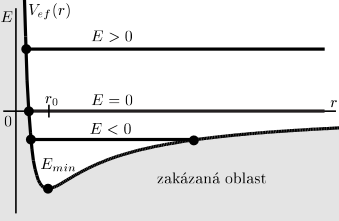
\includegraphics[width=210pt]{plot_1.png}
            }
            \item Binet's equation: $\frac{\d^2u}{\d\varphi^2} +u=-\frac{m}{L^2}\frac{\d V}{\d u}$ where $V(u)$ is a central potential and $u$ inverse distance. Solutions to $F(u)\sim u^3$ are Cotes spirals.
            \item $r=p/(1+\epsilon\cos\varphi)$, where $p=L^2/\alpha m$ and $\epsilon^2-1=2L^2E/\alpha^2m$.
            \item Full energy $K+\Pi$ of a body in a gravity field:$E=-GMm/2a$
            \item Vis-Viva equation: $v^2=GM\big(2/r - 1/a\big)$.
            \item For small eccentricities $\epsilon=f/a\ll 1$, trajectories can be considered as ahaving a circular shapes, with shifted foci.
            \item Properties of an ellipse: $l_1+l_2=2a$ ($l$ - distances from the foci), light from one focus is reflected to the other (angles with normal are same), $S=\pi ab$
            \item A circle and an ellipse with a focus at the circle's center can touch each other only at the longer axis.
            \item Gauss's law for gravity field $\vec g$:\\
            $\oint_{\partial V}\vec g\cdot\vec{dS}=-4\pi GM$ or $\nabla\cdot\vec g=-4\pi G\rho$\\
            $\oint_{\partial S}\vec g\cdot\vec{dl}=0$ or $\nabla\times\vec g=0$ (conservative field)
            \item Laplace-Runge-Lenz vector (LRL or the eccentricity vector), where $\alpha=GMm$ and $\epsilon=A/m\alpha$ $$\vec\epsilon=\frac{\vec v\times\vec L}{GMm}-\vec e_R\qquad\text{or}\qquad\vec A=\vec p\times\vec L-m\alpha\vec e_R$$
            \item Reduced mass: 2 body interaction lagrangian in CM: $\mathcal L=\mu\dot r^2/2+V(r)$, where $1/\mu=1/m_1+1/m_2$ is the reduced mass and $r$ is distance between them.
            \item Bertrand's theorem: only central forces $F\propto R^{-2}$ and $F\propto R$ (Harmonic osc.) give rise to closed orbits independently of initial conditions.
            \item Virial theorem for finite movement:\\
            If $F \propto r^n$, then $n\langle K \rangle = \langle \Pi \rangle$ (time avarages)
            \item Tsiolkovsky rocket equation:\\ $\Delta v=u\ln(M_{init}/M_{fin})$
            \item Rutheford scattering $\frac{\d\sigma }{\d\Omega}=\left(\frac {Q_1Q_2e^2}{8\pi\epsilon_0mv_\infty^2}\right)^2\frac{1}{\sin^4\frac{\theta }{2}}$
            \item {\color{red}add Tidal forces}
        \end{enumerate}

    \centering{\large\textbf{VIII. LAGRANGIAN FORMALISM}}
        \begin{enumerate}

            \item Generalized coordinate $q$: $\mathcal M\dot{q}^2/2+\Pi(q)=E$\\ $\mathcal M\ddot q =-\d\Pi(q)/\d q$ and $T =\mathcal M\dot{q}^2/2$
            \item Constraints are \textbf{a)} two-side $\phi=0$ or one-side $\phi\geq 0$, \textbf{b)} Scleronomic $\phi(q_i)=0$ or Reonomic $\phi(q_i,t)=0$, \textbf{c)} Holonomic $\phi(q_i,t)=0$ or non-holonomic (kinetic) $\phi(q_i,\dot q_i,t)=0$.
            \item Lagrange eqs. of 1st kind: $m\ddot x_i=F_i+T_i+\lambda\partial_i\phi$, where $\phi(x^j,t)=0$, $F_i$ is net ext. force and $T_i$ is net friction force. In vector notation:\\ $m\ddot{\vec x}=\vec F+\vec T+\lambda\nabla\phi$.
            \item Lagrange eqs. of 1st kind for $N$ particles and $V$ constraints: $m\ddot x_i=F_i+\sum_{v=1}^V\lambda^v\partial\phi_v/\partial x^i$ for $i\in\{1,\ldots, 3N\}$ and  $\phi_v(x^1,\ldots,x^{3N},t)=0$ for $v\in\{1,\ldots, V\}$.
            \item Stationary constrained particle under an action of force $\vec F$ obeys: $\vec F+\lambda\nabla\phi=0$ and $\vec F\times\nabla\phi=0$.
            \item Virtual work: in equilibrium\\ $\delta W=\delta \Pi-\sum_{i=1}^{3N}F_i\delta x^i =0$
            \item Differential principles: \textbf{a)} D'Alembert's principle: $\sum_{i=1}^{3N}(F_i-m\ddot x_i)\delta x^i=0$, \textbf{b)} Jourdain principle: $\sum_{i=1}^{3N}(F_i-m\ddot x_i)\delta\dot x^i=0$, \textbf{c)} Gauss's principle of least constraint: $\sum_{i=1}^{3N}(F_i-m\ddot x_i)\delta \ddot x^i=0$. All virtual displacements have to obey constraints and be reversible (for every $\delta x^i$ there exists $-\delta x^i$).
            \item D'Alembert's principle in geometrical form: $(m\ddot{\vec x}-\vec F)\cdot\vec t=0,\;\forall\vec t\in T_PQ$.
            \item D'Alembert's principle for all virtual displacements: $\sum_{i=1}^{3N}(m\ddot x_i-F_i-\sum_{v=1}^V\lambda_v\partial\phi_v/\partial x^i)\delta x^i=0$
            \item $\partial q^i/\partial\dot q^j=0=\partial\dot q^i/\partial q^j$, $\partial q^i/\partial q^j=\delta_j^i=\partial\dot q^i/\partial\dot q^j$
            \item Generalized force: $Q_j=\partial x^i/\partial q^jF_i$ and \\ $\frac{\d}{\d t}\left(\frac{\partial T}{\partial\dot q^j}\right)-\frac{\partial T}{\partial q^j}=Q_j=-\frac{\partial V}{\partial q^j}$
            \item Generalized potential of force $Q_j$:\\ $\frac{\d}{\d t}\left(\frac{\partial V}{\partial\dot q^j}\right)-\frac{\partial V}{\partial q^j}=Q_j$
            \item Lagrange's eqs. of 2nd kind: \\$\frac{\d}{\d t}\left(\frac{\partial L}{\partial\dot q^j}\right)-\frac{\partial L}{\partial q^j}=0$ where $L=T-\Pi$.
            \item $L$ is a function on $TQ$.
            \item Trajectory of system in $t\in[t_1,t_2]$ is such, that action $S=\int_{t_1}^{t_2}L(q^j(t),\dot q^j(t),t)\d t$ is stationary, $\delta S=0$.
            \item $f(q_j(t),\dot q_j(t))$ is an integral of motion if it is constant in time over the trajectory $q_j(t)$. ($\d f(t)/\d t=0$).
            \item If $q^i$ is a cyclic coordinate ($L$ is not a funct. of $q^i$), then $\partial L/\partial\dot q^i$ is an integral of motion.
            \item If $L$ is not a funct. of $t$, then generalized energy $h(q^i,\dot q^i)=\frac{\partial L}{\partial\dot q^j} \dot q^j-L$ is an integral of motion.
            \item If forces are conservative and constraints are both holonomic and ccleronomic, then $h=T+\Pi=const.$
            \item Lagrangian for a system of coupled oscillators: $L=\frac{1}{2}\left(T_{ij}\dot q_i\dot q_j-\Pi_{ij}q_iq_j\right)$ which yields $\tilde T\ddot{\vec q}-\tilde\Pi\vec q=0$ what can be solved using eigendecomposition.
            \item Euler-Ostrogradsky eq. for $L(y(x^i), y_{,i}(x^i), x^i)$:  \\$\sum_i\frac{\partial}{\partial x^i}\left(\frac{\partial L}{\partial y_{,i}}\right)-\frac{\partial L}{\partial y}=0$ where $y_{,i}=\partial y/\partial x^i$.
            \item Euler-Poisson eq. for $L(q^j, \dot q^j,\ldots,q^{(k)j}, t)$:  \\$-(-1)^k\frac{\d^k}{\d t^k}\left(\frac{\partial L}{\partial q^{(k)j}}\right)+\dots+\frac{\d}{\d t}\left(\frac{\partial L}{\partial\dot q^j}\right)-\frac{\partial L}{\partial q^j}=0$.
            \item Euler-Lagrange constrained eq. \\$\frac{\d}{\d t}\left(\frac{\partial(L+\lambda\phi)}{\partial\dot q^j}\right)-\frac{\partial(L+\lambda\phi)}{\partial q^j}=0$
            \item $S=\int_\Omega\mathcal L(\Phi,\Phi_{,\mu},x^\mu)\d\Omega$ where $\d\Omega=\d V\d t$ and $\mathcal L$ is Lagrangian density.
            \item $\frac{\partial}{\partial x^\mu}\left(\frac{\partial\mathcal L}{\partial\Phi_{,\mu}}\right)-\frac{\partial\mathcal L}{\partial\Phi}=0$
            \item Noether's theorem: if change of coord. $t'=t+\epsilon T(q^j, t)$,  $q'^j=q^j+\epsilon Q^j(q^j, t)$ does not change $L$, ($L(q^j(t), \dot q^j(t), t)=L'(q'^j(t'), \dot q'^j(t'), t')$) then the integral of motion is $\mathcal Z=\sum_j\frac{\partial L}{\partial\dot q^j}(Q^j-\dot q^jT)+LT$.
            \item $L+\d F/\d t$ where $F$ is any smooth function gives the same eqs. of motion as $L$.
            \item For EM. field $L=mv^2/2-e(\varphi-\vec v\cdot\vec A)$.
            \item Calibration of EM. fields: $\varphi'=\varphi-e^{-1}\partial F/\partial t$, $\vec A'=\vec A+e^{-1}\nabla F$.
            \item {\color{red} Add my coordinate transform of E-L equation.}
        \end{enumerate}

    \centering{\large\textbf{IX. HAMILTONIAN FORMALISM}}
        \begin{enumerate}
            \item Canonical (generalized) momentum: $p_j=\partial L/\partial\dot q^j$
            \item $\partial p_i/\partial q^j=0$, $\partial q^i/\partial q^j=\delta_{~j}^i$, $\partial p_i/\partial p_j=\delta_i^{~j}$
            \item The physical state of a system is given by a point in the phase space.
            \item Canonical variables $q^i$ and $p_i$ are implicit functs. of $t$: they depend on trajectory $q^i=q^i(\gamma(t))$, $p_i=p_i(\gamma(t))$. Hence $\partial q^i/\partial t=\partial p_i/\partial t= 0$.
            \item Every singular point in the phase space is a stable equilibrium state of the system.
            \item Hamiltonian is defined as $H(q^j,p_j,t)=\sum p_i\dot q^i-L(q^j,\dot q^i, t)$ where $\dot q^i=\dot q^i(q^j,p_j,t)$ is an inverse of $p_j=p_j(q^i, \dot q^i, t)$.
            \item $H$ is a function on $T^*Q$.
            \item Lagrange's and Hamilton's formalisms are equivalent $\Leftrightarrow$ if $L$ has no inflex points, $\det\left(\frac{\partial^2 L}{\partial\dot q^i\partial\dot q^j}\right)\neq 0$.
            \item $L(q^j,\dot q^j,t)=\sum p_i\dot q^i-H$ where $p_i$ is an inverse of $\dot q^i=\partial H/\partial p_i$.
            \item Hamilton's canonical equations: $\d q^i/\d t=\partial H/\partial p_i$ and $\d p_i/\d t=-\partial H/\partial q^i$.
            \item Legendre transformation: Let $I\subset\R$ be an interval, and $f:I\to\R$ a convex function; then its Legendre transform is the function $f^*:I^*\to\R$ defined by $f^*(x^*)=\sup_{x\in I}(x^*x-f(x))$ where $x^*\in I^*$.
            \item Legedre transformation $TQ\leftrightarrow T^*Q$ is given by $L(q^j,\dot q^i, t)\leftrightarrow H(q^j,p_j,t)$, hence $H=p_i\dot q^i-L\leftrightarrow L=p_i\dot q^i-H$ and $p_i=\partial L/\partial\dot q^i$, $\dot q^i=\partial L/\partial p_i$.
            \item Point mass in potential $V$:\\\textbf{a)} $H=\frac{1}{2m}(p_x^2+p_y^2+p_z^2)+V(x,y,z)$\\\textbf{b)} $H=\frac{1}{2m}(p_R^2+\frac{p_\theta^2}{R^2}+p_z^2)+V(R,\theta,z)$\\\textbf{c)} $H=\frac{1}{2m}(p_R^2+\frac{p_\vartheta^2}{R^2}+\frac{p_\varphi^2}{R^2\sin^2\vartheta})+V(R,\vartheta,\varphi)$
            \item For EM. field $H=(\vec p-e\vec A)^2/2m+e\varphi$.
            \item Poisson brackets: $\{f,g\}=\sum_i\left(\frac{\partial f}{\partial q^i}\frac{\partial g}{\partial p_i}-\frac{\partial f}{\partial p_i}\frac{\partial g}{\partial q^i}\right)$
            \item \textbf{a)} $\{f,g\}=-\{g,f\}$\\
                \textbf{b)} $\{c_1f_1+c_2f_2,g\}=c_1\{f_1,g\}+c_2\{f_2,g\}$\\
                \textbf{c)} $\{\{f,g\},h\}+\{\{g,h\},f\}+\{\{h,f\},g\}=0$\\
                \textbf{d)} $\{f,f\}=0$\\
                \textbf{e)} $\{fg,h\}=\{f,h\}g+f\{g,h\}$\\
                \textbf{f)} $\frac{\partial}{\partial t}\{f,g\}=\{\frac{\partial f}{\partial t},g\}+\{f,\frac{\partial g}{\partial t}\}$\\
            \item Fundamental Poisson brackets:\\$\{q^i,q^j\}=0$, $\{p_i,p_j\}=0$, $\{q^i,p_j\}=\delta^i_{~j}$
            \item $\{x_i,L_j\}=\epsilon_{ijk}x_k$, $\{p_i,L_j\}=\epsilon_{ijk}p_k$, $\{L_i,L_j\}=\epsilon_{ijk}L_k$ where $L_i=\epsilon_{ijk}x_jp_k$ is an angular mom.
            \item $\frac{\d f}{\d t}=\{f,H\}+\frac{\partial f}{\partial t}$
            \item Function $f(q^i,p_i)$ is an integral of motion if $\{f,H\}=0$.
		\item {\color{red} Constant of motion.}
            \item If $H$ is not a funct. of $t$, $H=H(q^i,p_i)$ is an integral of motion.
            \item If $f$ and $g$ are integrals of motion, then also $\{f,g\}$ is an integral of motion.
            \item $\d q^i/\d t=\{q^i,H\}$ and $\d p_i/\d t=\{p_i,H\}$
            \item $H(q^i,p_i,t)\to H'(Q^j(q^i,p_i,t),P_j(q^i,p_i,t),t)$ is a canonical transformation if it preserves the form of Hamilton's canonical eqs.
            \item Canonical transformations are generated by functions in 1st col. Requirements for canonicity are in 2nd col. and for integrability are in 3rd col.
            \begin{tabular}{|c|c|c|}
                \hline
                \rule{0pt}{3ex}
                $F_1(q^j,Q^j,t)$ & $\frac{\partial F_1}{\partial q^i}=p_i$ $\frac{\partial F_1}{\partial Q^k}=-P_k$ & $\frac{\partial p_i}{\partial Q^k}=-\frac{\partial P_k}{\partial q^i}$ \rule{0pt}{3ex}\\\hline
                \rule{0pt}{3ex}
                $F_2(q^j,P_j,t)$ & $\frac{\partial F_2}{\partial q^i}=p_i$ $\frac{\partial F_2}{\partial P_k}=Q^k$ & $\frac{\partial p_i}{\partial P_k}=\frac{\partial Q^k}{\partial q^i}$ \rule{0pt}{3ex}\\\hline
                \rule{0pt}{3ex}
                $F_3(p_j,Q^j,t)$ & $\frac{\partial F_3}{\partial p_i}=-q^i$ $\frac{\partial F_3}{\partial Q^k}=-P_k$ & $\frac{\partial q^i}{\partial Q^k}=\frac{\partial P_k}{\partial p_i}$ \rule{0pt}{3ex}\\\hline
                \rule{0pt}{3ex}
                $F_4(p_j,P_j,t)$ & $\frac{\partial F_4}{\partial p_i}=-q^i$ $\frac{\partial F_4}{\partial P_k}=Q^k$ & $\frac{\partial q^i}{\partial P_k}=-\frac{\partial Q^k}{\partial p_i}$ \rule{0pt}{3ex}\\\hline
            \end{tabular}
            First test if transformation is integrable (3rd col.), then find $F_a$ (2nd col.), finally use gen. funct. as
            $H'(Q^j,P_j,t)=H(q^j,p_j,t)+\partial F_a/\partial t$.
            \item Solving for generating function is analogic to solving for potential of conservative force.
            \item Generating functions $F_a$ are connected with Legendre dual transformation:
            $F_1(q,Q)$,\\$F_2(q,P)=F_1+P_iQ^i$,~~~~ $F_3(p,Q)=F_1-p_iq^i$,\\$F_4(p,P)=F_1+P_iQ^i-p_iq^i$.
            \item Transformation is canonical $\Leftrightarrow$\\ $\{Q^i,P_j\}=\delta^I_{~j}$ and $\{Q^i,Q^j\}=0=\{P_i,P_j\}$.
            \item Set of all canonical transformations is a group, which group operation is composition of two transformations.
            \item Poisson brackets are invariant under canonical transformations. $\{f,g\}_{q,p}=\{f,g\}_{Q,P}$
            \item Volume of phase-space is invariant under canonical transformations.
            \item Phase space distribution $\rho(p,q)$ determines the probability $\rho(p,q)\d^nq\d^np$ that the system will be found in the infinitesimal phase space volume $\d^nq\d^np$.
            \item Liouville theorem: the phase-space distribution function is constant along the trajectories of the system, $\partial\rho/\partial t+\{\rho,H\}=0$.
            \item {\color{red} Hamilton-Jacobbi theory}
        \end{enumerate}

    \centering{\large\textbf{X. PROPERTIES OF MATERIALS}}
        \begin{enumerate}
            \item Hooke's law: $\sigma=Y\epsilon=F/S$; where $\sigma$ is tensile stress, $\epsilon=\Delta L/L$ is extension, $Y=kL/S$ is Young's modulus;
            \item Energy density of deformation: $w=E/V=Y\epsilon^2/2$
            \item $l=l_0(1+\alpha\Delta T)$, $V=V_0(1+\beta\Delta T)$, $\rho=\rho_0(1-\beta\Delta T)$;\\for isotropic materials $\beta\approx 3\alpha$
            \item Speed of sound in elastic material: $c_s=\sqrt{Y/\rho}$
        \end{enumerate}

    \centering{\large\textbf{XI. FLUID MECHANICS}}
        \begin{enumerate}
		\item Pouzivaj stramlines ked nejde vyintegrovat rychlosti.
            \item Hydrostatic pressure: $p_h=h\rho g$; NB! atmospheric pressure $p=p_A+p_h$; Buoyancy: $F_B=V\rho g$, ($V$-sunked);
            \item Continuity equation: $S\rho v=const.$; Special case - continuity condition: $S\rho v=dm/dt$
            \item Bernoulli eq. - incompr. fluid: $p+\rho\varphi+\rho v^2/2=const.$\\In homog. fiels, in gravit. potential: $\varphi=gh$;
            \item Torricelli's law: $v=\sqrt{2gh}$ if Energy  is conserved or $v=\sqrt{gh}$ if momentum is conserved;
            \item Liquid surface takes equipot. shape (neglecting $\sigma$); in incompr. liquid: $p=p_0-w$, $w$ is vol. dens. of pot. en.
            \item Speed of shallow $(h\ll\lambda)$ water waves: $v=\sqrt{gh}$\\derivation via Bernoulli and Continuity eqs;
            \item Surface tension: $U=S\sigma$, $F=l\sigma$, $p=2\sigma/R$; Generally $p=\sigma\sum 1/R_i$ , In case of 2 surfaces $F$, $p$ times 2;
            \item Young-Laplace eq: $\Delta p=\sigma\nabla\cdot\vec n$
            \item Jurin's law: liquid height $h=2\sigma\cos\theta/\rho gr_0$\\$r_0$ - tube radius; $\theta$ - contact angle;
            \item Contact angle of droplet with the underlay:\\$\cos\theta=(\sigma_{SG}-\sigma_{SL})/\sigma_{GL}$
        \end{enumerate}

    \newpage
\end{multicols}
\end{document}
